\subsection{UC12 - Visualizzazione Riunioni Giornaliere }
\begin{itemize}
	\item \textbf{Identificativo}: UC12
	\item \textbf{Nome}: Visualizzazione Riunioni Giornaliere
	\item\textbf{Descrizione Grafica}: 
	\begin{figure}[h]
		\centering
		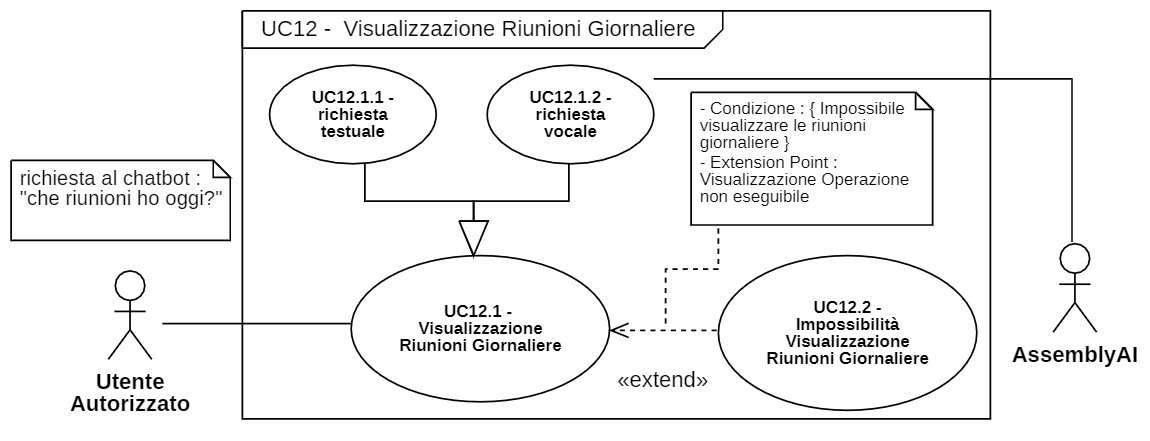
\includegraphics[scale=0.60]{images/UC12.png}
		\caption{Descrizione grafica caso d'uso UC12}
	 \end{figure}

	\item \textbf{Attori}
	\begin{itemize} 
		\item \textit{Primari}: Utente autorizzato e autenticato nella \glossario{piattaforma riunioni}
		\item \textit{Secondari}: Non presenti
	\end{itemize}
	\item \textbf{Descrizione}: L'utente richiede di visualizzare le Riunioni del giorno.
	\item \textbf{Precondizione}: L'utente ha effettuato il login sia sull'app che sulla piattaforma esterna, e si trova nella chat.
	\item \textbf{Postcondizione}: Il chatbot restituisce la lista delle riunioni del giorno, con eventuali informazioni.
	\item \textbf{Scenario principale}:  \begin{enumerate}
		\item Utente invia un messaggio al chatbot : "Che riunioni ho oggi?";
		\item Chatbot restituisce la lista delle riunioni, con eventuali informazioni.
	\end{enumerate}
\end{itemize}

\subsubsection{UC12.1 - Visualizzazione Riunioni Giornaliere }
\begin{itemize}
	\item \textbf{Identificativo}: UC12.1
	\item \textbf{Nome}: Visualizzazione Riunioni Giornaliere
	\item\textbf{Descrizione Grafica}: (Approfondita in UC12)
	\item \textbf{Attori}
	\begin{itemize} 
		\item \textit{Primari}: Utente autorizzato e autenticato nella \glossario{piattaforma riunioni}
		\item \textit{Secondari}: Non presenti
	\end{itemize}
	\item \textbf{Descrizione}: L'utente richiede di visualizzare le riunioni del giorno al chatbot.
	\item \textbf{Precondizione}: L'utente si è autenticato nell'app e nella \glossario{piattaforma riunioni} e si trova nella chat.
	\item \textbf{Postcondizione}: Il chatbot restituisce la lista delle riunioni del giorno, con eventuali informazioni.
	\item \textbf{Scenario principale}:  \begin{enumerate}
		\item Utente invia la richiesta al chatbot;
		\item Il chatbot visualizza la lista delle riunioni, con eventuali informazioni.
	\end{enumerate}
\end{itemize}

\paragraph{UC12.1.1 - Richiesta testuale }
\begin{itemize}
	\item \textbf{Identificativo}: UC12.1.1
	\item \textbf{Nome}: Richiesta testuale
	\item\textbf{Descrizione Grafica}: (Approfondita in UC12)
	\item \textbf{Attori}
	\begin{itemize} 
		\item \textit{Primari}: Utente autorizzato e autenticato nella \glossario{piattaforma riunioni}
		\item \textit{Secondari}: Non presenti
	\end{itemize}
	\item \textbf{Descrizione}: L'utente richiede di visualizzare le riunioni del giorno tramite input testuale.
	\item \textbf{Precondizione}: L'utente si è autenticato nell'app e nella \glossario{piattaforma riunioni} e vuole visualizzare le riunioni del giorno.
	\item \textbf{Postcondizione}: L'utente invia la richiesta in formato testuale.
	\item \textbf{Scenario principale}:
	\begin{enumerate}
		\item L'utente vuole visualizzare le riunioni del giorno;
		\item L'utente inserisce testualmente la richiesta.
	\end{enumerate}
\end{itemize}

\paragraph{UC12.1.2 - Richiesta vocale }
\begin{itemize}
	\item \textbf{Identificativo}: UC12.1.2
	\item \textbf{Nome}: Richiesta vocale
	\item\textbf{Descrizione Grafica}: (Approfondita in UC12)
	\item \textbf{Attori}
	\begin{itemize} 
		\item \textit{Primari}: Utente autorizzato e autenticato nella \glossario{piattaforma riunioni}
		\item \textit{Secondari}: Non presenti
	\end{itemize}
	\item \textbf{Descrizione}: L'utente richiede di visualizzare le riunioni del giorno tramite input vocale.
	\item \textbf{Precondizione}: L'utente si è autenticato nell'app e nella \glossario{piattaforma riunioni} e vuole visualizzare le riunioni del giorno.
	\item \textbf{Postcondizione}: L'utente invia la richiesta in formato vocale.
	\item \textbf{Scenario principale}:
	\begin{enumerate}
		\item L'utente vuole visualizzare le riunioni del giorno;
		\item L'utente inserisce attraverso input vocale la richiesta.
	\end{enumerate}
\end{itemize}

\subsubsection{UC12.2 - Impossibilità visualizzazione Riunioni Giornaliere }
\begin{itemize}
	\item \textbf{Identificativo}: UC12.2
	\item \textbf{Nome}: Impossibilità visualizzazione Riunioni Giornaliere
	\item\textbf{Descrizione Grafica}: (Approfondita in UC12)
	\item \textbf{Attori}
	\begin{itemize} 
		\item \textit{Primari}: Utente autorizzato e autenticato nella \glossario{piattaforma riunioni}
		\item \textit{Secondari}: Non presenti
	\end{itemize}
	\item \textbf{Descrizione}: L'utente richiede di visualizzare le riunioni del giorno ma viene restituito un messaggio d'errore.
	\item \textbf{Precondizione}: L'utente si è autenticato nell'app e nella \glossario{piattaforma riunioni} e si trova nella chat.
	\item \textbf{Postcondizione}: Il chatbot risponde con un messaggio d'errore indicando l'impossibilità di effettuare l'operazione.
	\item \textbf{Scenario principale}: L'utente richiede di vedere le riunioni giornaliere, ma gli viene negato e visualizza un messaggio d'errore.
\end{itemize}
\newpage